% Chapter Template

\chapter{Ensayos y resultados} % Main chapter title

\label{Chapter4} % Change X to a consecutive number; for referencing this chapter elsewhere, use \ref{ChapterX}

%----------------------------------------------------------------------------------------
%	SECTION 1
%----------------------------------------------------------------------------------------
En este capítulo se explica la metodología de pruebas aplicada tanto a los componentes individuales como al sistema implementado, para finalizar con una comparación con el estado del arte.


\section{Banco de pruebas}
\label{sec:Banco de pruebas}
%
La verificación del correcto funcionamiento de los módulos que componen el sistema se realizó mediante una maqueta que se muestra en la figura \ref{fig:maqueta} y representa el invernadero del cliente en escala reducida.

\begin{figure}[H]
	\centering
	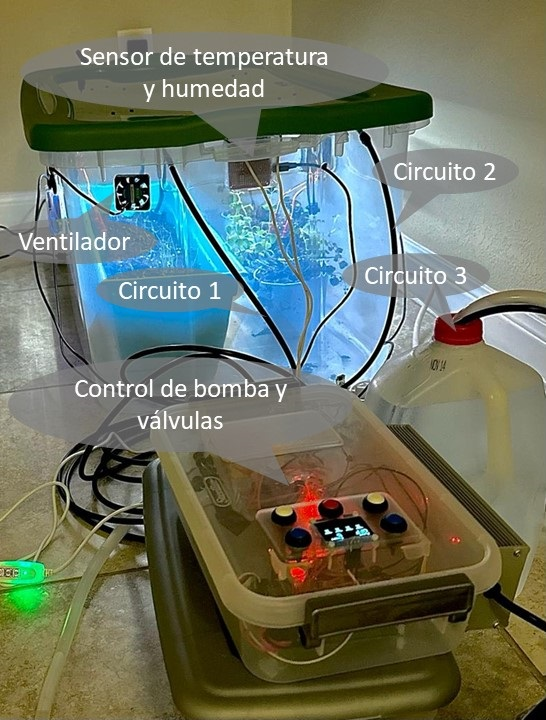
\includegraphics[width=0.50\textwidth]{./Figures/chapter4/maqueta.jpg}
	\caption[Modelo completo del invernadero]{Modelo completo del invernadero.}
	\label{fig:maqueta}
\end{figure}

El modelo cuenta con una bomba de agua conectada a tres válvulas para alimentar los circuitos de riego en los que se utilizaron mangueras neumáticas y conexiones de aluminio de acople rápido. El conjunto armado puede verse en la figura \ref{fig:pump}. 
  
El ensamblado se muestra en las figuras \ref{fig:gh1}, \ref{fig:gh2} y \ref{fig:gh3} donde se observa la implementación de dos circuitos de riego independientes. También se configuró un tercer circuito cerrado para pruebas de accionamiento de bomba y válvula a fin de evitar desperdicios durante las fases de calibración.



Además se incorporaron a la maqueta dos módulos sensores de humedad del suelo, uno de temperatura y humedad y un actuador para el encendido de los ventiladores.

Las pruebas manuales de accionamiento de los diferentes sistemas y las de acceso concurrente a la aplicación central se realizaron mediante una computadora portátil y un teléfono celular.

\begin{figure}[htpb]
     \centering
       \begin{subfigure}[b]{0.45\textwidth}
	    \centering
		 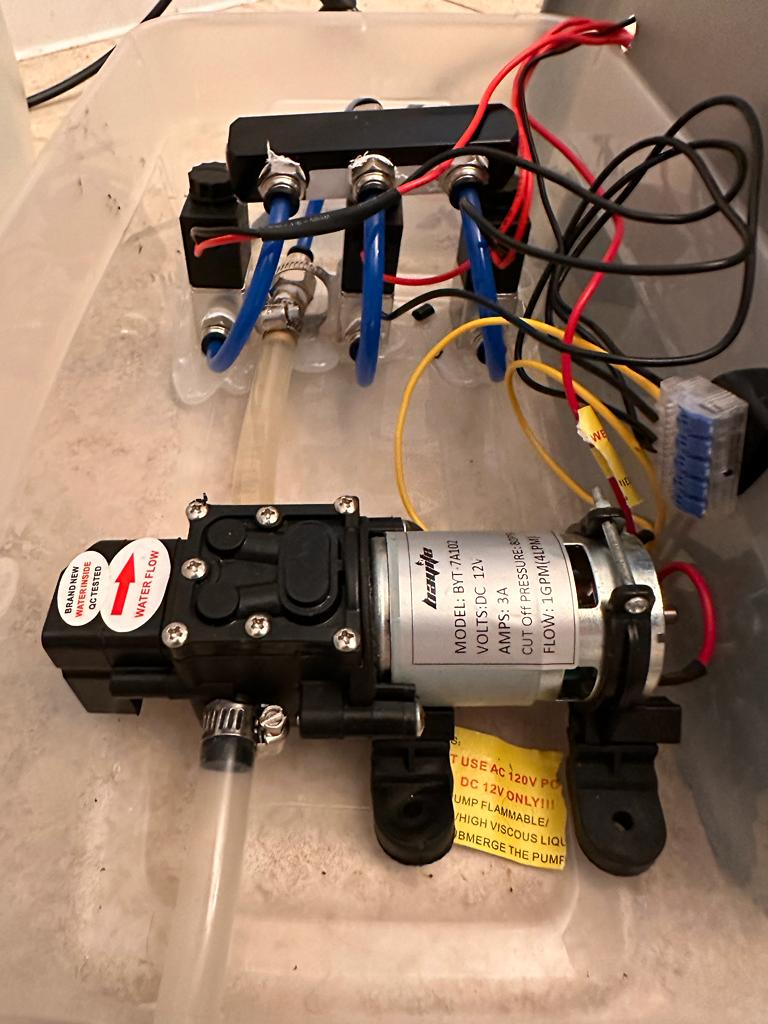
\includegraphics[width=0.75\textwidth]{./Figures/chapter4/pump_2.jpg}
		\caption{Conjunto bomba y válvulas.}
		\label{fig:pump}
     \end{subfigure}
          \hfill
     \begin{subfigure}[b]{0.45\textwidth}
		\centering
		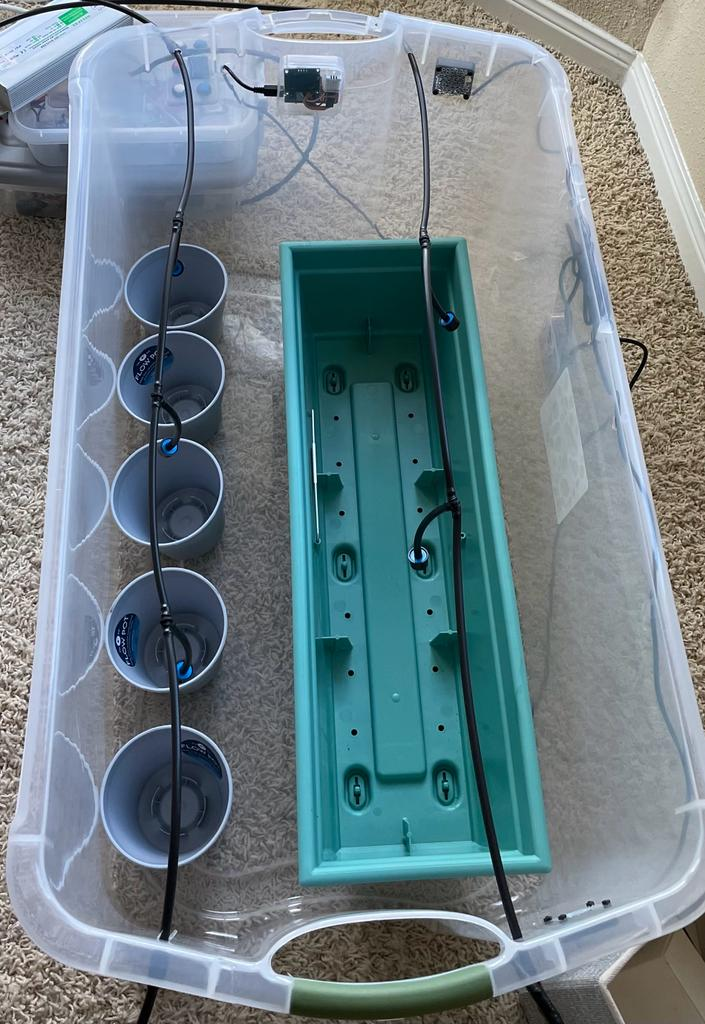
\includegraphics[width=0.70\textwidth]{./Figures/chapter4/Invernadero1.jpg}
		\caption{Armado de mangueras de riego.}
		\label{fig:gh1}
     \end{subfigure}
     \hfill
     \begin{subfigure}[b]{0.45\textwidth}
	    \centering
		 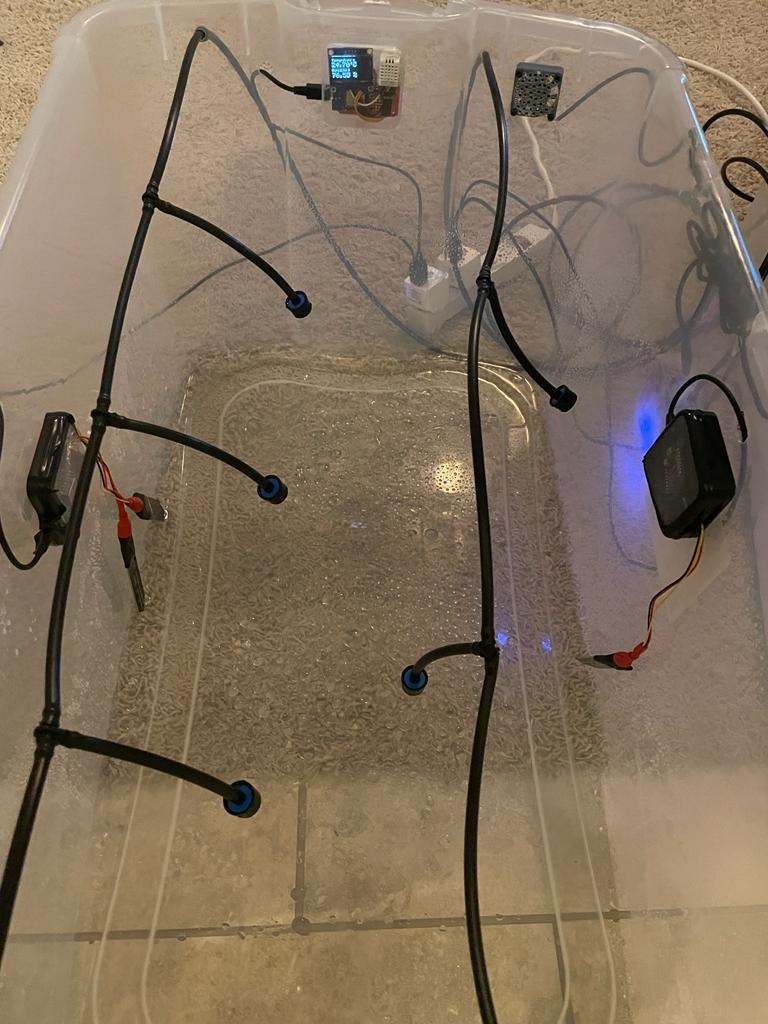
\includegraphics[width=0.75\textwidth]{./Figures/chapter4/Invernadero2.jpg}
		\caption{Pruebas de riego.}
		\label{fig:gh2}
     \end{subfigure}
     \hfill	
	 \begin{subfigure}[b]{0.45\textwidth}
		\centering
		\includegraphics[width=0.65\textwidth]{./Figures/chapter4/Invernadero3.jpg}
		\caption{Ensamble general.}
		\label{fig:gh3}
     \end{subfigure}
     \hfill

        \caption[Modelo de pruebas del invernadero]{Modelo de pruebas del invernadero.}
        \label{fig:invernadero}
\end{figure}



\pagebreak
\section{Pruebas individuales}
\label{sec:Pruebas individuales}

Se detallan las principales pruebas realizadas a los módulos a fin de garantizar su correcto funcionamiento y/o el cumplimiento de requerimientos.


\subsection{Pruebas a módulos sensores}
\label{sec:Pruebas a módulos sensores}

\begin{itemize}
\item Conexión a los sensores y valores obtenidos: se conectaron individualmente los módulos a la computadora mediante la consola serial de Arduino IDE y se constataron los valores obtenidos frente a cambios inducidos sobre la magnitud a medir.


\item Conexión a la aplicación y envío de telemetría: se cargó el firmware en los módulos sensores conforme a lo descrito en las secciones \ref{Firmware módulos sensores de humedad del suelo} y \ref{Firmware módulo sensor de temperatura y humedad}, mientras que se configuró la instancia instalada de ThingsBoard de acuerdo a lo explicado en \ref{sec:Configuración de la aplicación}. Se construyó un \textit{dashboard} (tablero de visualización) en donde se incluyeron los \textit{widgets} (componentes visuales) necesarios para visualizar la telemetría en tiempo real.
Desde la consola serial del módulo, se comprobó la  conexión del microcontrolador a la red Wi-Fi. Posteriormente se verificó la vinculación del dispositivo con la aplicación y se constató la correcta recepción de los valores en el \textit{dashboard}. La figura \ref{fig:dashboard} muestra una captura de pantalla de las series de tiempo correspondientes.

\begin{figure}[!h]
	\centering
	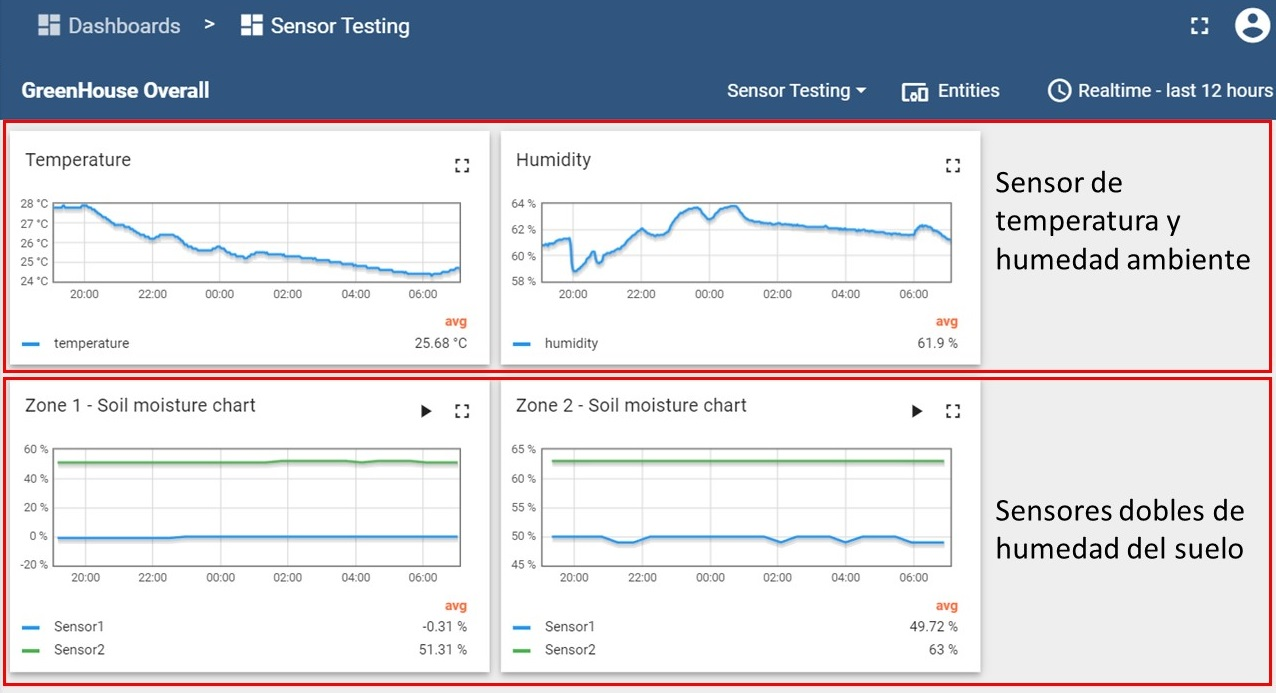
\includegraphics[width=0.90\textwidth]{./Figures/chapter4/dashboard.jpg}
	\caption[\textit{Dashboard} de visualización de telemetría]{\textit{Dashboard} de visualización de telemetría.}
	\label{fig:dashboard}
\end{figure}


%\item Sincronización  y control de dispositivos mediante atributos compartidos: Para comprobar la correcta comunicación entre la aplicación y TB, se crearon atributos de configuracion como los valores minimos y maximos que pueden ser leidos por un sensor de humedad del suelo. luego se creo un dashboard en TB para poder modificar esos valores, y se comprobo en el disposivo la correcta recepcion de los mismos por consola serial.


\item Sincronización de los sensores de humedad: como se indicó en la sección \ref{Protocolos de comunicación}, la comunicación con la aplicación central es bidireccional. Para constatar la correcta recepción de mensajes por parte del módulo, se establecieron atributos compartidos capaces de ser modificados desde ThingsBoard. Por medio de  un \textit{dashboard} se realizaron variaciones de los valores de calibración de los sensores y diferentes tiempos para el \textit{deep sleep}.
Se comprobó la recepción de los parámetros por consola serial y la acción en consecuencia por parte del módulo.
En la figura \ref{fig:soil_calib} se observa el estado de humedad del suelo en dos sensores, los valores de ajuste y la configuración del tiempo de hibernación.

\begin{figure}[!h]
	\centering
	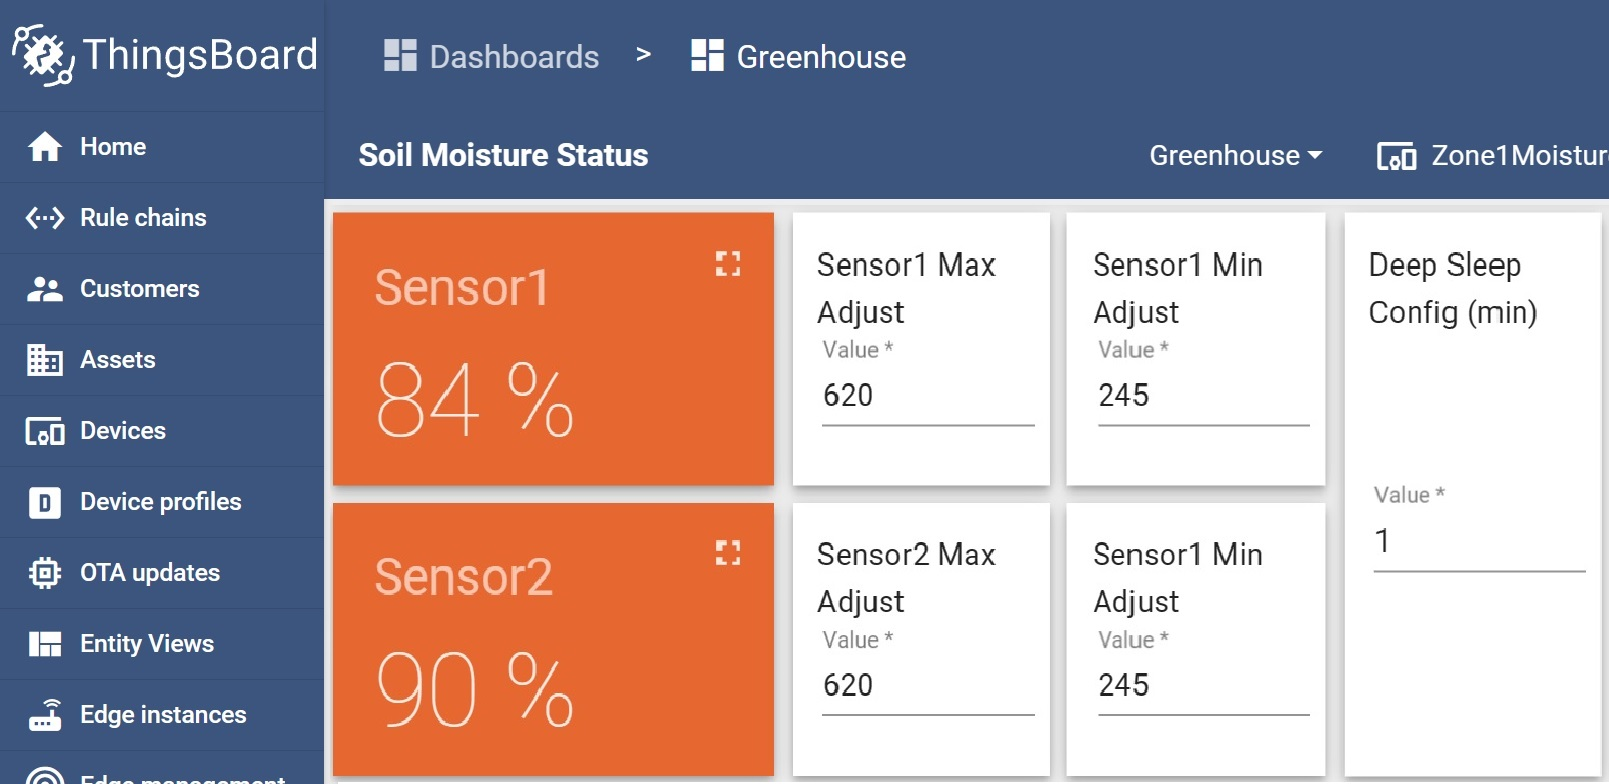
\includegraphics[width=0.80\textwidth]{./Figures/chapter4/soil_calib.jpg}
	\caption[Atributos de sensores de humedad del suelo]{Atributos de sensores de humedad del suelo.}
	\label{fig:soil_calib}
\end{figure}

\item Resistencia al agua y a salpicaduras: requerimiento la prueba sobre este requerimiento no funcional consistió en comprobar la integridad y el funcionamiento del módulo al tiempo que se sumergía el sensor en un recipiente con agua o se lo sometía a aspersiones continuas durante alrededor de 30 segundos con atomizadores desde diferentes ángulos.
La figura \ref{fig:soil_test} esquematiza parcialmente el proceso de prueba mencionado.

\begin{figure}[h]
	\centering
	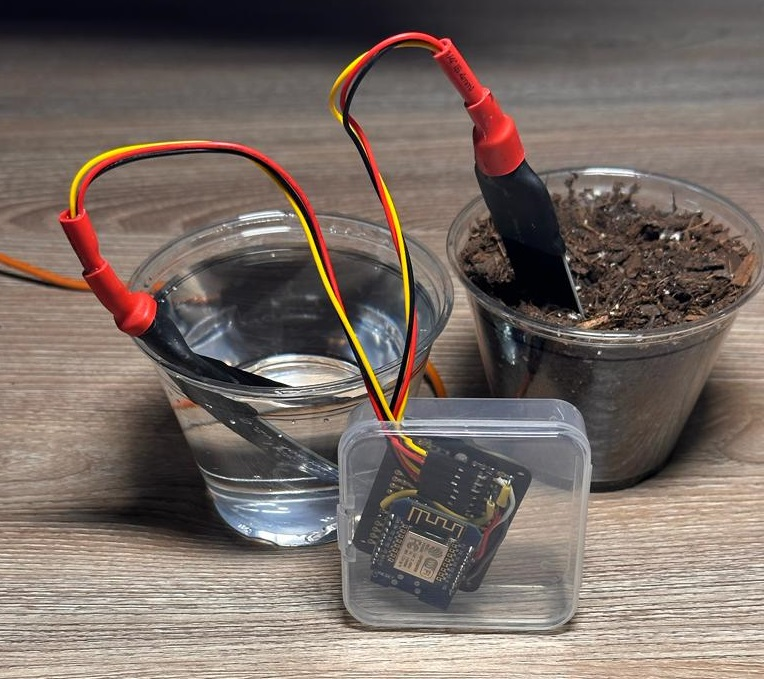
\includegraphics[width=0.50\textwidth]{./Figures/chapter4/soil_testing3.jpg}
	\caption[Prueba de resistencia al agua]{Prueba de resistencia al agua.}
	\label{fig:soil_test}
\end{figure}
  
\end{itemize}








\subsection{Pruebas a módulos actuadores}
\label{sec:Pruebas a módulos actuadores}

Se conectaron las salidas de los pines de GPIO a leds para visualizar el encendido y apagado del actuador. 

La figura \ref{fig:control_test1} muestra la interfaz desarrollada en ThingsBoard a fin de enviar las señales de comando al módulo por medio de mensajes RPC sobre MQTT. El microcontrolador recibe la orden y ejecuta la acción, reflejada en el estado de los leds correspondientes como se observa en la figura \ref{fig:control_test2}.



\begin{figure}[htpb]
     \centering
       \begin{subfigure}[b]{0.50\textwidth}
	    \centering
		 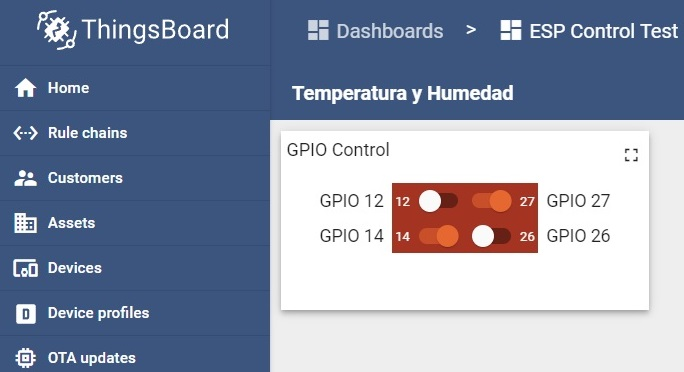
\includegraphics[width=0.9\textwidth]{./Figures/chapter4/control_unit_test_1.jpg}
		\caption{Ventana de control.}
		\label{fig:control_test1}
     \end{subfigure}
          \hfill
     \begin{subfigure}[b]{0.45\textwidth}
		\centering
		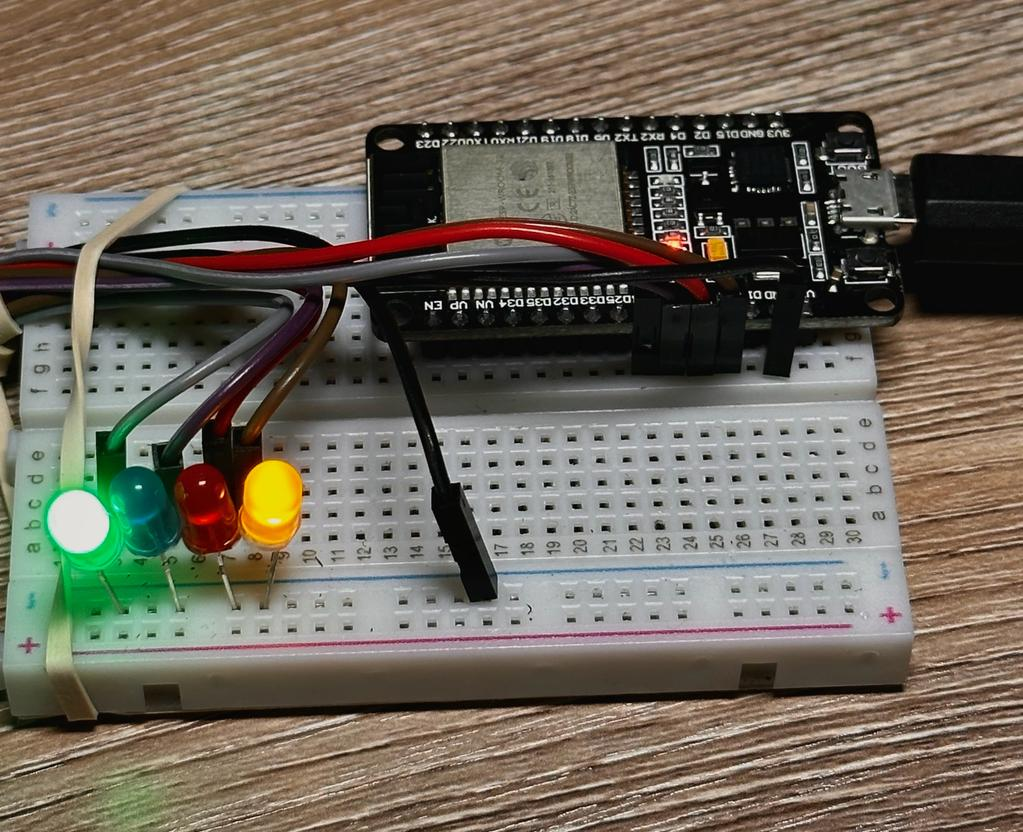
\includegraphics[width=0.70\textwidth]{./Figures/chapter4/control_test2.jpg}
		\caption{Verificación del actuador mediante leds.}
		\label{fig:control_test2}
     \end{subfigure}
     \hfill
        \caption[Pruebas unitarias sobre controladores]{Pruebas unitarias sobre controladores.}
        \label{fig:control_test}
\end{figure}


\subsection{Pruebas de acceso concurrente a la aplicación}
\label{sec:Pruebas de acceso concurrente a la aplicación}



Las pruebas de concurrencia se efectuaron mediante el acceso simultáneo de diferentes usuarios desde la computadora y el teléfono celular. Los ensayos consistieron en realizar distintas acciones desde un dispositivo como, por ejemplo, el accionamiento de un circuito de riego por parte de un usuario, y la confirmación del cambio de estado recibida por otro. 
 
La figura \ref{fig:tb_compu} muestra la vista obtenida mediante el uso del ordernador mientras que la figura  \ref{fig:tb_celu}, la del celular.

\begin{figure}[htpb]
     \centering
       \begin{subfigure}[b]{0.53\textwidth}
	    \centering
		 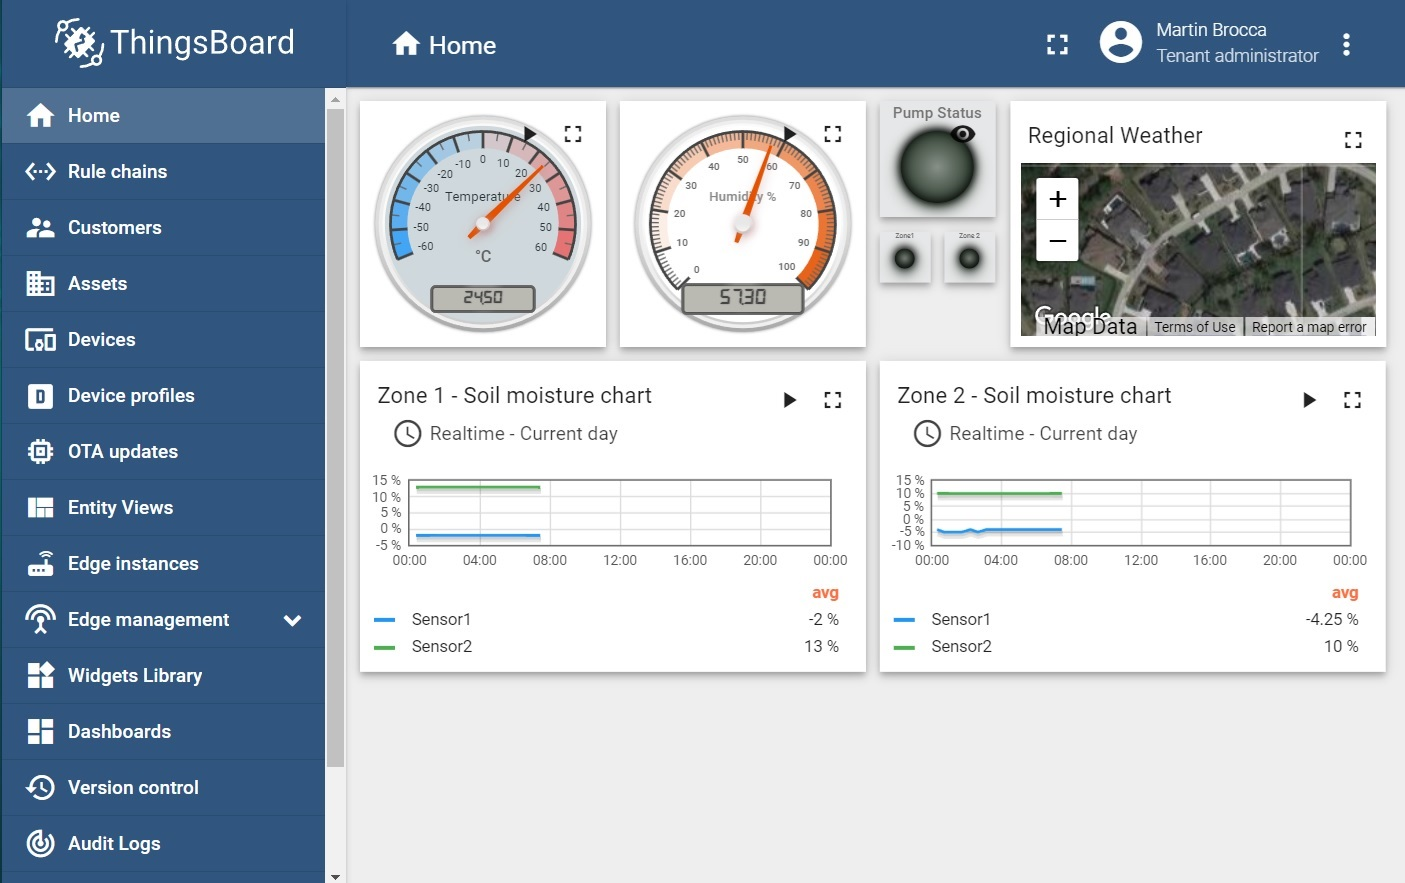
\includegraphics[width=0.9\textwidth]{./Figures/chapter4/tb_compu.jpg}
		\caption{Vista del acceso por computadora.}
		\label{fig:tb_compu}
     \end{subfigure}
          \hfill
     \begin{subfigure}[b]{0.45\textwidth}
		\centering
		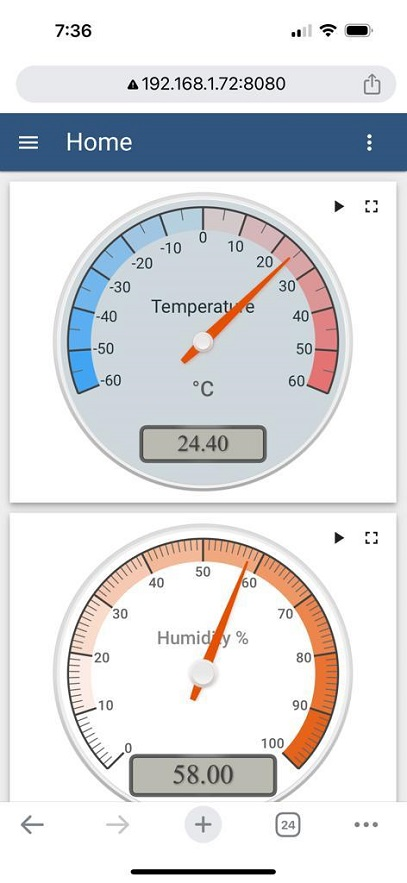
\includegraphics[width=0.40\textwidth]{./Figures/chapter4/tb_celu.jpg}
		\caption{Vista del acceso por teléfono celular.}
		\label{fig:tb_celu}
     \end{subfigure}
     \hfill
        \caption[Pruebas unitarias de acceso concurrente]{Pruebas unitarias sobre acceso concurrente.}
        \label{fig:tb_concurrencia}
\end{figure}

\section{Pruebas de integración}
\label{sec:Pruebas de sistema}

Tienen por objetivo verificar el correcto funcionamiento e interacción de los sistemas que conforman el modelo. Con este propósito se desarrollaron reglas de automatización para el control de riego y temperatura, además de las necesarias para el manejo de alarmas del sistema. 

Estas reglas, cuyo esquema se muestra en la figura \ref{fig:basic_rule}, son similares en construcción y constan de los siguientes nodos y relaciones:

\begin{itemize}
\item Recepción de mensajes desde los módulos sensores.
\item Identificación del emisor en base a los metadatos del mensaje.
\item Lectura de la telemetría.
\item Comparación con valor de referencia.
\item[] Si la comparación resulta exitosa, dispara una alerta de notificación al cliente e informa al microcontrolador que comience una acción. En caso contrario, limpia cualquier alerta presente y de ser necesario, detiene la acción en el actuador.
\end{itemize}





\begin{figure}[h]
	\centering
	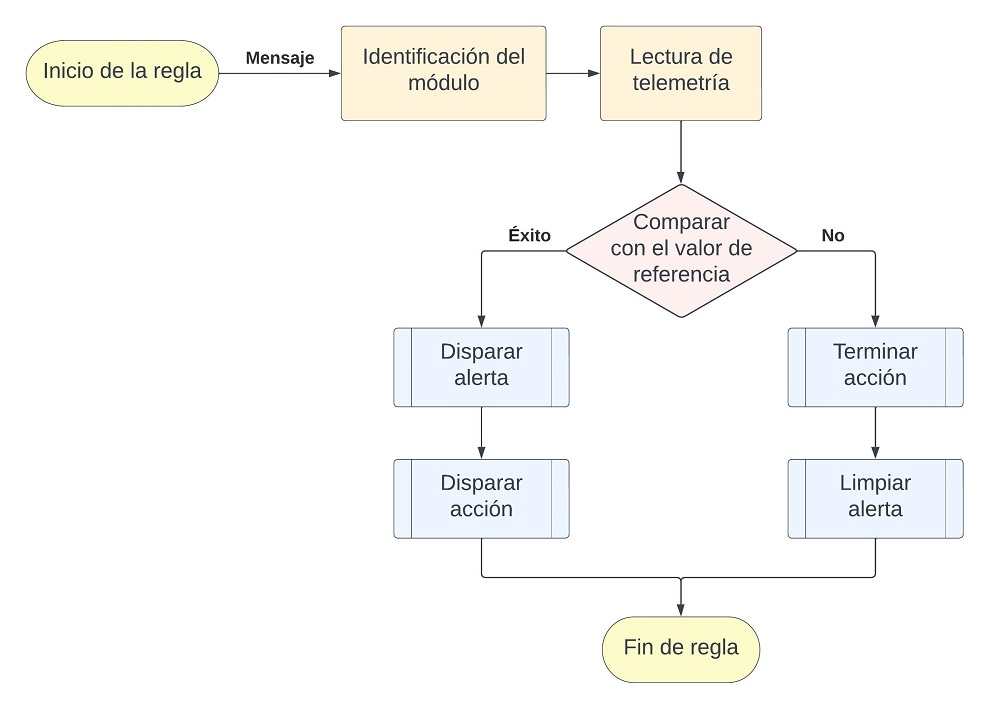
\includegraphics[width=0.8\textwidth]{./Figures/chapter4/ReglaBasica.jpg}
	\caption[Regla de automatización genérica]{Regla de automatización genérica.}
	\label{fig:basic_rule}
\end{figure}

\pagebreak

\subsection{Control de clima}
\label{sec:Control de clima}

Se definió una regla de control con un límite máximo de 28 °C de temperatura que, cuando se supera, envía un mensaje de encendido de ventiladores e inicia el proceso de notificación  al usuario. Por el contrario, si la temperatura se mantiene por debajo del umbral, se cancelan las alarmas y retorna al estado de espera de mensajes. La regla implementada se muestra en la figura \ref{fig:temp_rule}.  

\begin{figure}[h]
	\centering
	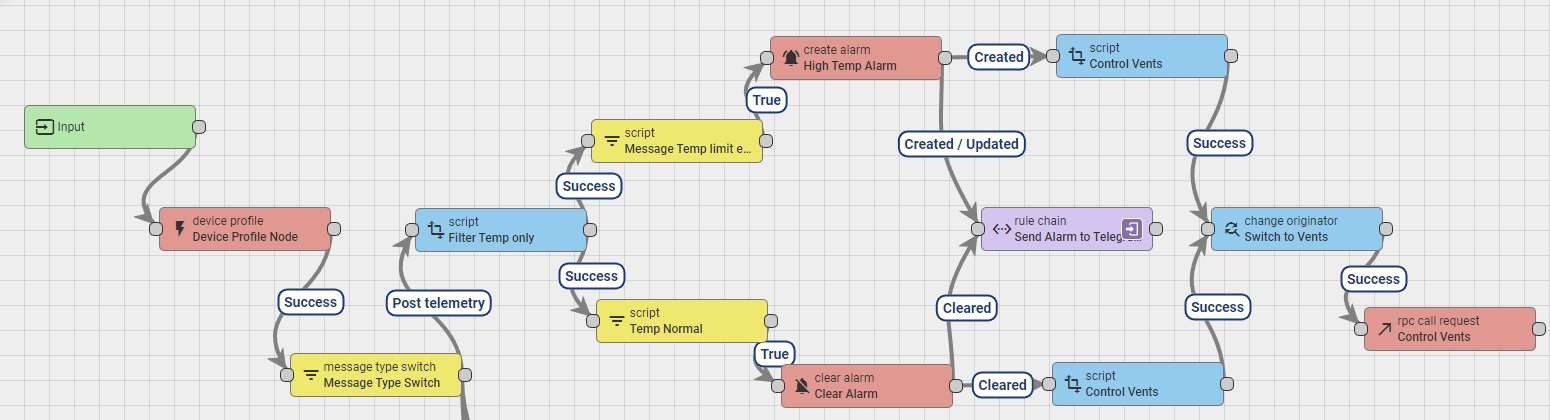
\includegraphics[width=1\textwidth]{./Figures/chapter4/temp_rule.jpg}
	\caption[Regla de control de clima]{Regla de control de clima.}
	\label{fig:temp_rule}
\end{figure}

Para la prueba se instaló la maqueta en un entorno de ambiente controlado a 25 °C para luego incrementar la temperatura artificialmente por medio de una pistola de calor y observar la reacción del sistema. La figura \ref{fig:temp_graph} corresponde al diagrama histórico de temperatura y humedad del invernadero. En el recuadro rojo se muestra el instante en donde el cambio de temperatura dispara la acción del sistema y se encienden los ventiladores, mientras que en las figuras \ref{fig:temp_alarm} y \ref{fig:temp_alarm_user} se observan las alarmas del dispositivo y de usuario creadas por este evento.  







%\begin{figure}[h]
%	\centering
%	\includegraphics[width=0.7\textwidth]{./Figures/chapter4/ventrule.jpg}
%	\caption[Regla de automatización de ventilador]{Regla de automatización de ventilador.}
%	\label{fig:temp_rule}
%\end{figure}


\begin{figure}[!h]
     \centering
       \begin{subfigure}[b]{0.8\textwidth}
	    \centering
		 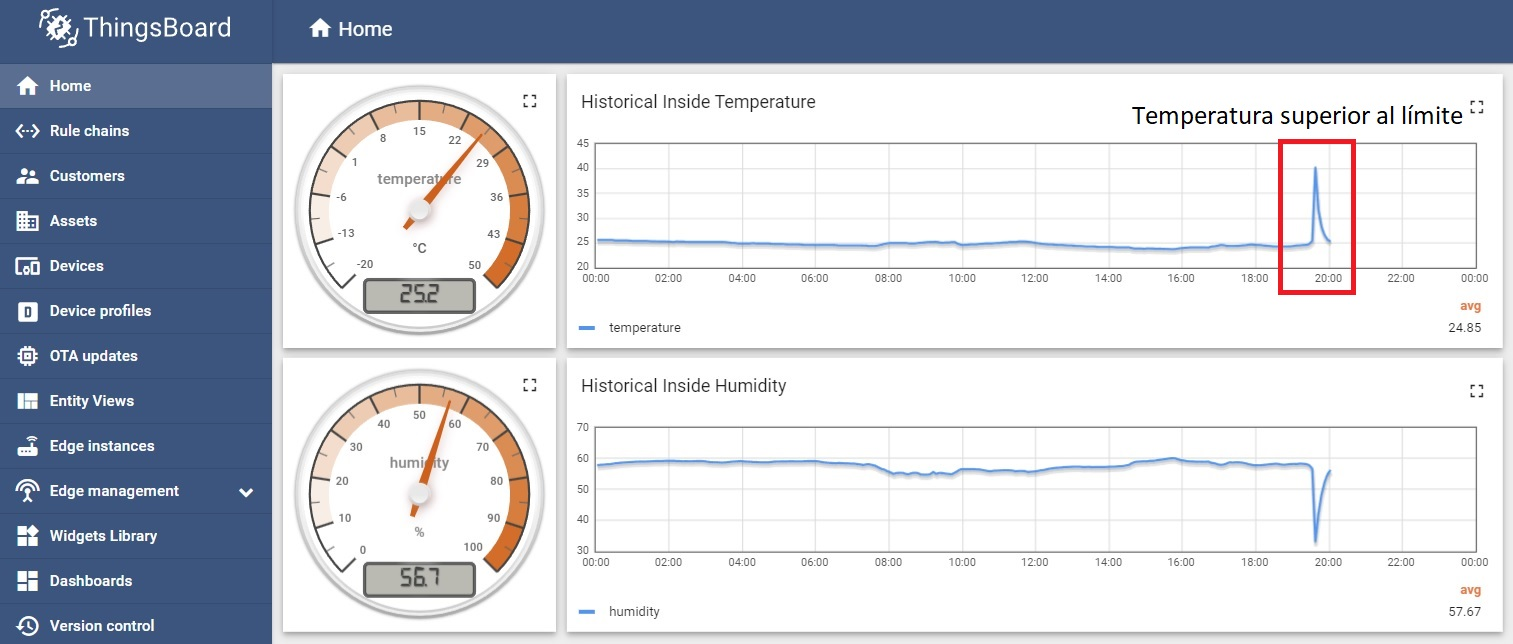
\includegraphics[width=0.9\textwidth]{./Figures/chapter4/temperature.jpg}
		\caption{Vista del historial de temperatura.}
		\label{fig:temp_graph}
     \end{subfigure}
          \hfill
     \begin{subfigure}[b]{0.50\textwidth}
		\centering
		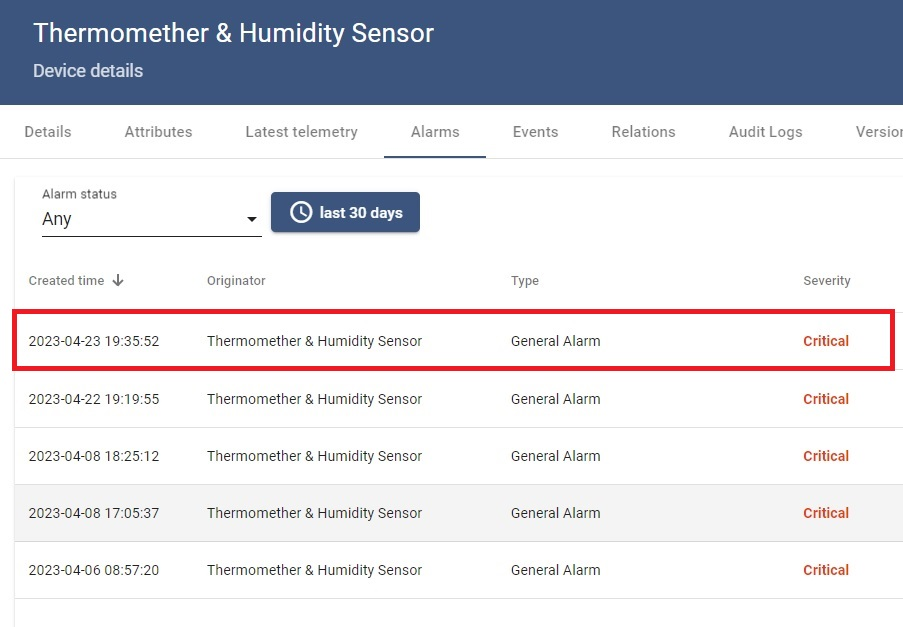
\includegraphics[width=1\textwidth]{./Figures/chapter4/temp_alarm.jpg}
		\caption{Alarmas en el dispositivo.}
		\label{fig:temp_alarm}
     \end{subfigure}
     \begin{subfigure}[b]{0.45\textwidth}
		\centering
		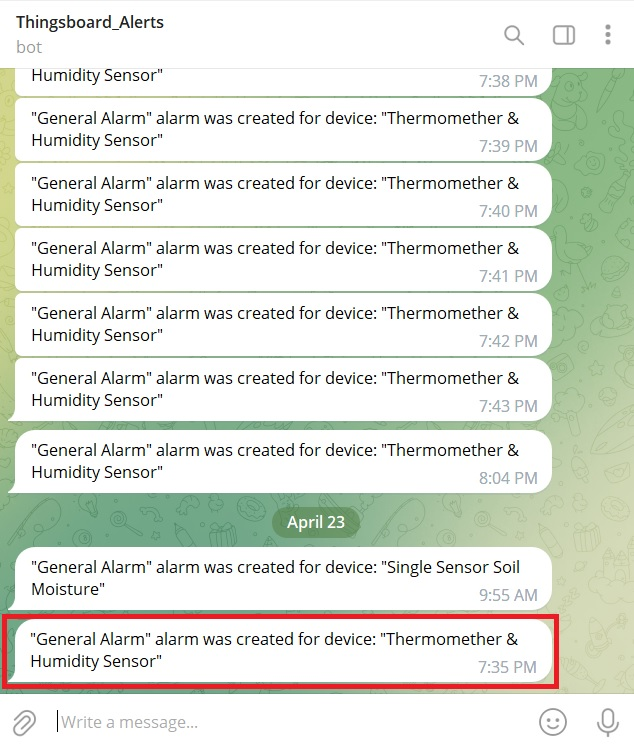
\includegraphics[width=0.80\textwidth]{./Figures/chapter4/temp_user_alarm.jpg}
		\caption{Alarma recibida por el usuario.}
		\label{fig:temp_alarm_user}
     \end{subfigure}
     \hfill
        \caption[Generación de alarmas por exceso de temperatura]{Generación de alarmas por exceso de temperatura.}
        \label{fig:tb_clima_automation}
\end{figure}


\pagebreak
\subsection{Control de riego}
\label{sec:Control de riego}

La prueba de integración del sistema de riego se realizó sobre la maqueta descripta en la sección  \ref{sec:Banco de pruebas} empleando un módulo sensor doble por circuito de riego. La utilización de dos sondas por módulo pretende que el riego sea uniforme sobre diferentes disposiciones de macetas. 

Se construyó una regla de control según lo descrito en la sección \ref{sec:Pruebas de sistema} donde se reciben las lecturas provenientes desde los dos módulos sensores. Como primer paso, se identifica la zona a la que pertenecen las sondas. Si el valor recibido es inferior a la referencia, corresponde a un suelo seco, por lo tanto se debe iniciar el sistema de bomba y válvula correspondiente al circuito por el tiempo de riego predefinido.


Para evaluar la regla se plantearon los siguientes parámetros de configuración de sensor:
\begin{itemize}
\item Seco: sonda expuesta al aire, limpia y sin rastros de humedad.
\item Húmedo: sensor introducido en tierra con una humedad aproximada del 35\%.
\end{itemize}

En la tabla \ref{tab:tb_riego} se registró el resultado de las diferentes pruebas realizadas, considerando estas exitosas solamente cuando en ambos sensores del módulo se indique un suelo seco y se dispare el sistema de riego para el sector correspondiente.
La figura \ref{fig:soil_graph} muestra el gráfico histórico de humedad de suelo en donde se indica el instante en que ambas sondas se encuentran por debajo del umbral configurado y la correspondiente alarma generada se muestra en la figura \ref{fig:soil_alarm}.


\begin{table}[!h]
  \centering
  \caption[Pruebas de sistema de riego]{Pruebas de sistema de riego.}
  \begin{tabular}{llllccc}
  \toprule
  \multicolumn{2}{c}{\textbf{Zona 1}} &
    \multicolumn{2}{c}{\textbf{Zona 2}} &
    \multicolumn{1}{c}{\multirow{2}{*}{\textbf{\begin{tabular}[c]{@{}c@{}}Riego \\ zona 1\end{tabular}}}} &
    \multicolumn{1}{c}{\multirow{2}{*}{\textbf{\begin{tabular}[c]{@{}c@{}}Riego \\ zona 2\end{tabular}}}} &
    \multicolumn{1}{c}{\multirow{2}{*}{\textbf{Resultado}}} \\ %\cline{1-4}
  \textbf{Sensor 1} &
  \textbf{Sensor 2} &
  \textbf{Sensor 1} &
  \textbf{Sensor 2} &
  \multicolumn{1}{c}{} &
  \multicolumn{1}{c}{} &
  \multicolumn{1}{c}{} \\ \midrule
Seco	&Seco	&Seco	&Seco	&Activa	&Activa	&Ok \\
Seco	&Seco	&Seco	&Húmedo	&Activa	&No	&Ok \\
Seco	&Seco	&Húmedo	&Húmedo	&Activa	&No	&Ok \\
Seco	&Húmedo	&Seco	&Seco	&No	&Activa	&Ok \\
Seco	&Húmedo	&Seco	&Húmedo	&No	&No	&Ok \\
Seco	&Húmedo	&Húmedo	&Húmedo	&No	&No	&Ok \\
Húmedo	&Húmedo	&Seco	&Seco	&No	&Activa	&Ok \\
Húmedo	&Húmedo	&Seco	&Húmedo	&No	&No	&Ok \\
Húmedo	&Húmedo	&Húmedo	&Húmedo	&No	&No	&Ok \\
  \bottomrule
  \hline
  \end{tabular}
\label{tab:tb_riego}
\end{table}



\begin{figure}[!h]
     \centering
       \begin{subfigure}[b]{0.8\textwidth}
	    \centering
		 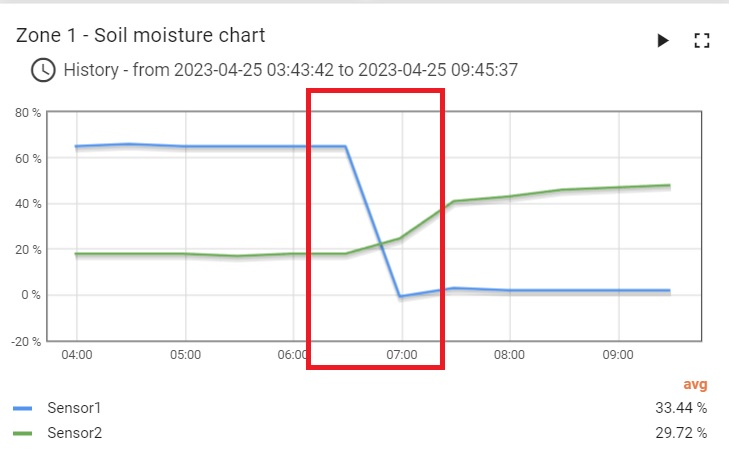
\includegraphics[width=0.9\textwidth]{./Figures/chapter4/soil_chart.jpg}
		\caption{Vista del historial de humedad del suelo.}
		\label{fig:soil_graph}
     \end{subfigure}
          \hfill
     \begin{subfigure}[b]{0.80\textwidth}
		\centering
		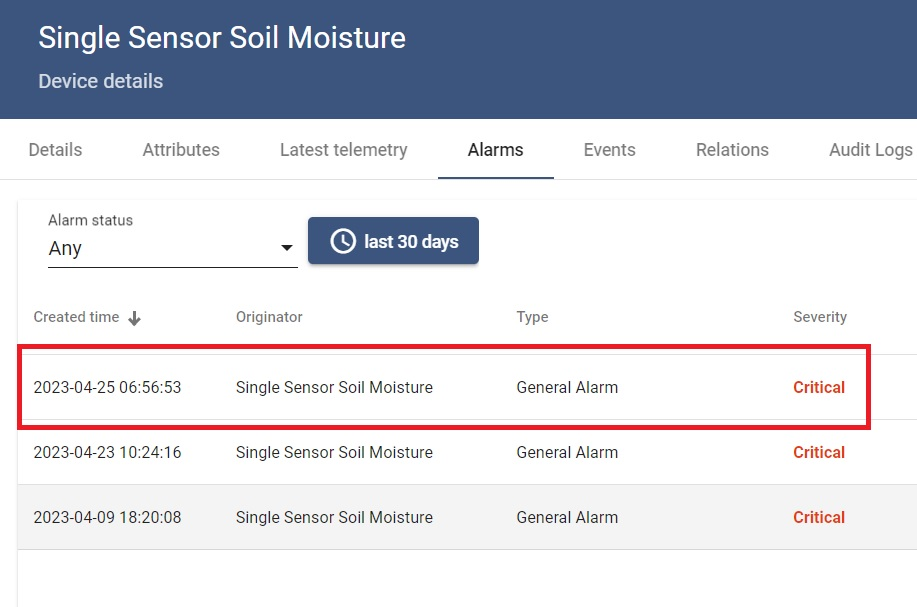
\includegraphics[width=0.80\textwidth]{./Figures/chapter4/soil_alarm.jpg}
		\caption{Alarmas generadas al superar los límites.}
		\label{fig:soil_alarm}
     \end{subfigure}
     \hfill
        \caption[Prueba del sistema de riego]{Prueba del sistema de riego.}
        \label{fig:tb_riego}
\end{figure}

\pagebreak
\section{Comparativa con el estado del arte}
\label{sec:Comparativa con el estado del arte}

El proyecto realizado permite corroborar que el desarrollo de un invernadero inteligente de tipo hogareño es capaz de satisfacer los requerimientos iniciales a pesar de las limitaciones de conexión a Internet y presupuesto del cliente.   


El trabajo resultante es asequible, personalizable y con posibilidades de expansión, pero requiere conocimientos en diversos dominios que incluyen los sistemas informáticos, la electrónica y la botánica, entre otros. En contrapartida, las soluciones comerciales ofrecen una amplia gama de características integradas, son más fáciles de instalar y configurar, pero son más costosas y menos adaptables.

En la tabla \ref{tab:comp_arte} se muestran las principales diferencias entre el proyecto realizado y las soluciones comerciales existentes.


%
%\begin{table}[htbp]
%    \centering
%	\caption[Comparación con el estado del arte]{Comparación con el estado del arte.}
%    %\begin{tabularx}{\textwidth}{sbb }
%    \begin{tabular}{>{\raggedright}p{0.19\textwidth} p{0.36\textwidth} p{0.36\textwidth}}
%%	\begin{tabular}{p{0.6\hsize} p{1.2\hsize} p{1.2\hsize}}
%
%%	\begin{tabular} {cll}
%        \toprule
%%        Característica  & Trabajo realizado & Soluciones comerciales \\ 
%		\multicolumn{1}{c}{\textbf{Característica}} &
%  		\multicolumn{1}{c}{\textbf{Trabajo realizado}} &
%  		\multicolumn{1}{c}{\textbf{Soluciones comerciales}} \\
%        \midrule
%    Costo           & Accesible, con gran variedad de productos disponibles en el mercado. & Costos medios a altos, con soluciones que dependen del producto seleccionado. \\
%    Personalización & Altamente personalizable y ajustable a las necesidades del usuario.  & Limitaciones en cuanto a la personalización.                                 \\
%    Capacidad de expansión &   Mayor flexibilidad para ser ampliado y personalizado con la incorporación de nuevos módulos de sensores y dispositivos. &    Limitaciones en cuanto a la expansión y personalización, aunque puede ofrecer más opciones de integración con otros sistemas. \\
%    Dificultad de instalación y ajustes & Requiere conocimientos técnicos para su instalación y configuración, pero puede ser más fácil de ajustar y personalizar. & Más fáciles de instalar y configurar, aunque puede requerir un período de aprendizaje para personalizar y ajustar a las necesidades específicas del usuario. \\
%    Funcionalidades e integración & Posee una limitada cantidad de funcionalidades integradas, aunque permite el desarrollo de las mismas. & Poseen una amplia gama de funcionalidades e integración con productos propios. \\ 
%    \bottomrule
%    \hline
%    \end{tabular}
%    \label{tab:comp_arte}
%\end{table}

\begin{table}[htbp]
    \centering
	\caption[Comparación con el estado del arte]{Comparación con el estado del arte.}

\begin{tblr}{
 column{1}={0.19\textwidth}, column{2}={0.36\textwidth}, column{3}={0.36\textwidth},
 rowsep=3pt,
 hline{1} = {0.8pt,solid}, 
 hline{2} = {0.6pt,solid}, 
 hline{7} = {1.3pt,solid},
 colspec = {X[l]X[l]X[l]},
 row{1} = {font=\bfseries}, rowhead = 1,
 } 
 Característica	&	Trabajo realizado	 &	Soluciones comerciales \\
 Costo           & Accesible, debido a la gran cantidad de componentes electrónicos y módulos disponibles en el mercado. & Costos medios a altos, con soluciones que dependen del producto seleccionado. \\
    Personalización & Altamente ajustable a las necesidades del usuario.  & Limitada.  \\
    Capacidad de expansión &   Mayor flexibilidad para ser ampliado y adaptado con la incorporación de nuevos módulos de sensores y dispositivos. &    Opciones supeditadas al fabricante. \\
    Dificultad de instalación y ajustes & Requiere conocimientos técnicos para su instalación y configuración. & Más fáciles de instalar y configurar, aunque pueden requerir una curva de aprendizaje para adecuarse a las necesidades específicas del usuario. \\
    Funcionalidades e integración & Posee una limitada cantidad de funcionalidades integradas, aunque permite su desarrollo. & Poseen una amplia gama de funcionalidades e integración con productos propios. \\ 
\end{tblr}
    \label{tab:comp_arte}
\end{table}